%!TeX root = main.tex
% TODO; wie darf ich einen meromorphen verändern, (das P verändern) ohne das
% sich effektiv was ändert?
% TODO: \cM = \cM_K ... replace
% TODO: Dimension eines meromorphen Zusammenhang
\chapter{Meromorphe Zusammenhänge}
\begin{comment}
Sei $\cM$ ein $\cD$-Modul ungleich Null von endlichem Typ. Falls die
links-Multiplikation mit $x$ bijektiv ist, so nennen wir $\cM$ einen
meromorphen Zusammenhang. \cite[Chap 4]{sabbah_cimpa90}
%TODO: erklären, erwähnen oder entfernen!
\end{comment}

\begin{comment}
\cite[Chap 5.1.1]{hotta2007d} %abgeschrieben
\end{comment}
Wir beginnen mit der klassischen Theorie von Gewöhnlichen
Differentialgleichungen.
Sei $V$ ein geeigneter Funktionenraum, beispielsweise der Raum der holomorphen
Funktionen.
%TODO: posibly multivalued
\begin{defn}[Systeme von ODEs]
Für eine Matrix $A=(a_{ij}(x))_{ij}\in M(n\times n,K)$
\footnote{
Es bezeichnet $M(n\times m,k)$ die Menge der $n$ mal
$m$ dimensionalen Matrizen mit Einträgen in $k$.
}
definieren wir das
\emph{System von gewöhnlichen Differentialgleichungen (kurz System von ODEs)}
als
\begin{equation}
\label{eq:KlassischesODE}
%TODO: partial oder d
\frac{d}{dx}u(x)=Au(x) \,,
\end{equation}
wobei $u(x)=\,^t(u_1(x),\dots,u_n(x))$ ein
Spaltenvektor\footnote{Für $v=(v_1,\dots,v_n)$ ein Vektor, bezeichnet
$ \,^tv:= \begin{pmatrix} v_{1}\\ \vdots\\ v_{n} \end{pmatrix} $
den transponierten Vektor.} von unbekannten Funktionen.
Wir sagen $v(x)=\,^t(v_1(x),\dots,v_n(x))$ ist eine \emph{Lösung} von
(\ref{eq:KlassischesODE}), falls $ v_i\in V$ für alle
$i\in\{1,\dots,n\}$ und $v$ die Gleichung (\ref{eq:KlassischesODE}), auf einer
Umgebung um die $0$, erfüllt.
\end{defn}

Durch setzen von $w(x)=Tu(x)$ für eine invertierbare Matrix $T\in GL(n,K)$
erhält man aus \ref{eq:KlassischesODE} das System 
\[
\frac{d}{dx}w(x)=(T^{-1}AT - T^{-1}\frac{d}{dx}T)w(x) \,,
\]
und deshalb erhalten wir die folgende Definition.
\begin{defn}[Differenziell Äquivalent]
Man nennt $A$ und $B\in M(n\times n,K)$ \emph{(differenziell) äquivalent}
($A\sim B$) genau dann, wenn es ein $T\in GL(n,K)$ gibt, mit
$B=T^{-1}AT-T^{-1}\frac{d}{dx}T$.
Dementsprechend sind zwei Systeme von ODEs äquivalent, wenn ihre zugeordneten
Matrizen differenziell äquivalent sind.
\end{defn}

\begin{comment}
$1=TT^{-1}$ $\rightsquigarrow$ $T'T^{-1}+T(T^{-1})'=0$\\
$1=T^{-1}T$ $\rightsquigarrow$ $(T^{-1})'T+T^{-1}T'=0$
\end{comment}

Mit elementarer Theorie über Gewöhnliche Differentialgleichungen lässt sich
ein System von ODEs in eine einzige ODE der Form
\begin{equation} \label{eq:UmgeformteODE}
(\underset{=:P}{\underbrace{ a_n\partial_x^n + a_{n-1}\partial_x^{n-1} +
  \cdots + a_1\partial_x + a_0}})\cdot u(t)=0 \,,
\end{equation}
mit $a_i\in K$ für alle $i\in\{0,\dots,n\}$, umschreiben. Dieses so erhaltene
$P\in\cD_K$ ist ein sogenannter linearer Differentialoperator und es gilt
\begin{align*}
v(x) \text{ ist Lösung von } P\cdot u(x)=0
&&\Rightarrow && \forall Q\in \cD_K \text{ ist } v(x) \text{ Lösung von }
QP\cdot u(x)=0 \,.
\end{align*}
Also ist eine Lösung von $P\cdot u(x)=0$ auch eine Lösung von $Q\cdot u(x)=0$
für alle $Q\in\cD_K\cdot P\vartriangleleft \cD_K$.

\begin{comment}
Sei $P$ ein linearer Differentialoperator mit Koeffizienten in $a_i(x)\in\Ckx$
geschrieben als $P=\sum^{d}_{i=0}{a_{i}(x)\partial_x^i}$.
Man sagt eine Funktion $u\in\cF$ ist Lösung von $P$, falls $u$ die Gleichung
$Pu=0$ erfüllt.
Man sagt $0$ ist ein singulärer Punkt falls $a_d(0)=0$.
Falls $0$ kein singulärer Punkt ist, hat $P$ genau $d$ über $\C$ Unabhängige
Lösungen in $\Ckx$. %TODO: oder \tilde\cO
\end{comment}

\section{Meromorphe Zusammenhänge}
Nun wollen wir dieses klassische Gebilde nun in die moderne Sprache der
meromorphen Zusammenhänge übersetzen.
%Quelle ist \cite{sabbah_cimpa90}
\begin{defn}[Meromorpher Zusammenhang] \label{def:merom-zush}
Ein \emph{meromorpher Zusammenhang} (bei $x=0$) ist ein Tupel
$(\cM_K,\partial)$ und besteht aus folgenden Daten:
\begin{itemize}
\item $\cM_K$, ein endlich dimensionaler $K$-Vektor Raum
\item einer $\C$-linearen Abbildung $\partial:\cM_K\rightarrow \cM_K$,
genannt \emph{Derivation} oder \emph{Zusammenhang}, welche für alle $f\in K$
und $u\in \cM_K$ die \emph{Leibnitzregel}
\begin{equation}\label{eq:Leibnitzregel}
\partial(fu)=f'u+f\partial u %TODO: hier klammern um das letzte u ?
\end{equation}
erfüllen soll.
\end{itemize}
\end{defn}
\begin{bem} %[Formaler meromorpher Zusammenhang]
Analog definiert man einen \emph{formalen meromorphen Zusammenhang}
$(\cM_{\hat K},\partial)$ bestehend, analog wie in Definition
\ref{def:merom-zush}, aus folgenden Daten:
\begin{itemize}
\item $\cM_{\hat K}$, ein endlich dimensionaler $\hat K$-Vektor Raum
\item einer $\C$-linearen Derivation $\partial:\cM_{\hat K}\rightarrow
\cM_{\hat K}$, welche die \emph{Leibnitzregel} (\ref{eq:Leibnitzregel})
erfüllen soll.
\end{itemize}
\end{bem}

\begin{bem}
Später wird man auf die Angabe von $\partial$ verzichten und einfach $\cM_K$
als den meromorphen Zusammenhang bezeichnen, auch wird manchmal auf die Angabe
von $K$ im Subscript verzichtet, sofern klar ist, welches $K$ gemeint ist.
\end{bem}

\begin{defn}
Seien $(\cM,\partial_\cM)$ und $(\cN,\partial_\cN)$ zwei meromorphe
Zusammenhänge über $k$. Eine $k$-lineare Abbildung $\phi:\cM\rightarrow\cN$
ist ein Morphismus von meromorphen Zusammenhängen, falls sie
$\phi\circ\partial_\cM=\phi\circ\partial_\cN$ erfüllt. In diesem Fall
schreiben wir auch $\phi:(\cM,\partial_\cM)\rightarrow(\cN,\partial_\cN)$.
Ein solcher Morphismus ist ein Isomorphismus, falls die Abbildung
$\phi:\cM\rightarrow\cN$ ein Isomorphismus von $k$-Vektorräumen ist.
\end{defn}

\begin{defn}
Wir erhalten damit die Kategorie der meromorphen Zusammenhänge über $k$ mit
\begin{align*}
\text{Objekte: } & (M,\partial)\text{ meromorpher Zusammenhang über }k
\\\text{Morphismen: } & (M,\partial)\overset{f}{\rightarrow}(M',\partial')
  \text{ Morphismus von meromorphen Zusammenhängen.}
\end{align*}
\end{defn}

\begin{lem} Sei $\cM_K$ ein endlich dimensionaler $K$-Vektor Raum mit
$\partial_1$ und $\partial_2$ zwei darauf definierte Derivationen, so gilt, die
Differenz zweier Derivationen ist $K$-linear.
\end{lem}
\begin{proof}
Seien $\partial_1$ und $\partial_2$ zwei Derivationen auf $\cM_K$.
Da $\partial_1$ und $\partial_2$ $\C$-linear, ist $\partial_1-\partial_2$
$\C$-linear, also muss nur noch gezeigt werden, dass
$(\partial_1-\partial_2)(fu)=f\cdot(\partial_1-\partial_2)(u)$ $\forall f\in
K$ und $u\in\cM_K$ gilt.\\
%TODO: wieso gilt das?
\begin{align*}
(\partial_1-\partial_2)(fu) &= \partial_1(fu)-\partial_2(fu)\\
&= f'u+f\partial_1u-f'u-f\partial_2u\\
&= \underset{=0}{\underbrace{f'u-f'u}}+f\cdot(\partial_1u-\partial_2u)\\
&= f\cdot(\partial_1-\partial_2)(u)\\
\end{align*}
\end{proof}
\begin{comment}
\begin{cor}
Für $(K^r,\partial)$ ein meromorpher Zusammenhang existiert ein $A\in M(r\times
r,K)$, so dass $\partial=\frac{d}{dx}-A$.
\end{cor}
\begin{proof}
Es sei $(K^r,\partial)$ ein meromorpher Zusammenhang.  So ist
$\frac{d}{dx}-\partial:K^r\rightarrow K^r$ $K$-linear, also lässt sich durch
eine Matrix $A\in M(r\times r,K)$ darstellen
%$\frac{d}{dx}-\partial=A$
, also ist, wie
behauptet, $\partial=\frac{d}{dx}-A$.
\end{proof}
\end{comment}

\begin{comment}
\cite[Seite 129]{hotta2007d}
\end{comment}
\begin{defn}[Zusammenhangsmatrix]
Sei $(\cM_K,\partial)$ ein meromorpher Zusammenhang so wähle eine $K$-Basis
$\{e_i\}_{i\in\{1,\dots,n\}}$ von $\cM$. Dann ist die
\emph{Zusammenhangsmatrix bzgl. der Basis $\{e_i\}_{i\in\{1,\dots,n\}}$} die
Matrix $A=(a_{ij}(x))_{i,j\in\{1,\dots,n\}}\in M(n\times n,K)$ definiert
durch
%\[ \partial e_j=-\sum_{i=1}^na_{ij}(x)e_i \,. \]
\[ a_{ij}(x) = -^te_i \partial e_j \,. \]
\end{defn}

Damit ist, bezüglich der Basis $\{e_i\}_{i\in\{1,\dots,n\}}$, die Wirkung von
$\partial$ auf $u=:\,^t(u_1,\dots,u_n)$ beschrieben durch
\iffalse
  \[
  \partial(u) = \partial \Big( \sum_{i=1}^nu_i(x)e_i \Big)
  =\sum_{i=1}^n \Big( u_i'(x)-\sum_{j=1}^na_{ij}u_j(x) \Big)e_i \,.
  \]
\fi
\begin{align*}
\partial(u) &= \partial \Big( \sum_{i=1}^nu_i(x)e_i \Big)
\\&=\sum_{i=1}^n \Big( u_i'(x)-\sum_{j=1}^na_{ij}u_j(x) \Big)e_i
\\&=\underbracket{\sum_{i=1}^n u_i'(x)e_i} 
  - \underbracket{\sum_{i=1}^n\sum_{j=1}^na_{ij}u_j(x)e_i}
\\&=\overbracket{u'(x)} 
  - \overbracket{Au(x)}
\end{align*}
Damit ist die Bedingung $\partial u(x)=0$, für $u(x)= \sum_{i=1}^n u_ie_i$,
äquivalent zu der Gleichung
\begin{equation*}
u'(x)=Au(x)
\end{equation*}
für $u(x)=\,^t(u_1(x),\dots,u_n(x))$. Damit haben wir gesehen,
dass jeder meromorphe Zusammanhang $(\cM,\partial)$ ausgestattet mit einer
$K$-Basis $\{e_i\}_{i\in\{1,\dots,n\}}$ von $\cM$ zu einem System von
gewöhnlichen Differentialgleichungen zugeordnet werden kann.

\begin{comment}
\begin{prop}[Transformationsformel] \cite[Chap 5.1.1]{hotta2007d}
In der Situation
\begin{center}
\begin{tikzpicture} [scale=3.3, descr/.style={fill=white,inner sep=2.5pt} ]
\matrix (m) [
  matrix of math nodes
  , row sep=3em
  , column sep=3em
  %, text height=3em
  %, text depth=0.25em
]
{
  K^r &   &   & K^r \\
      & M & M & \\
  K^r &   &   & K^r \\
};
\path[->,font=\scriptsize,>=angle 90]
(m-1-1) edge node[descr]{$\cong$} node[above]{$\phi$} (m-2-2)
(m-3-1) edge node[descr]{$\cong$} node[above]{$\psi$} (m-2-2)
(m-1-4) edge node[descr]{$\cong$} node[above]{$\phi$} (m-2-3)
(m-3-4) edge node[descr]{$\cong$} node[above]{$\psi$} (m-2-3)

(m-2-2) edge node[above]{$\partial$} (m-2-3)

(m-1-1) edge node[above]{$\frac{d}{dz}+A$} (m-1-4)
(m-3-1) edge node[above]{$\frac{d}{dz}+B$} (m-3-4)

(m-3-1) edge node[descr]{$\cong$} node[right]{$T$} (m-1-1)
(m-3-4) edge node[descr]{$\cong$} node[left]{$T$} (m-1-4)
;

\path[>=stealth,|->]
;
\end{tikzpicture}
\end{center}
mit $\phi,\psi$ und $T$ $K$-Linear und $\partial,(\frac{d}{dx}+A)$ und
$(\frac{d}{dx}+B)$ $\C$-Linear, gilt:\\
Der meromorphe Zusammenhang. $\frac{d}{dx}+A$ auf $K^r$ wird durch
Basiswechsel
$T\in GL(r,K)$ zu
\[
\frac{d}{dx}+(T^{-1}\cdot T'+T^{-1}AT) = \frac{d}{dx}+B
\]
\end{prop}
\end{comment}

\begin{defn}
Wenn wir umgekehrt mit einer Matrix $A=(a_{ij}(x))\in M(n\times n,K)$,
welche eine System von ODEs beschreibt, beginnen, können wir durch
\begin{align*}
\cM_A & :=\bigoplus_{i=1}^n Ke_i &&\text{und}
& \partial_A \sum_{i=1}^n u_ie_i &:= \sum_{i=1}^n\left(
  \frac{\partial u_i}{\partial x}-\sum_{j=1}^na_{ij}(x)u_j \right)e_i
\end{align*}
den \emph{assoziierten meromorphen Zusammenhang} $(\cM_A,\partial_A)$ definieren.
\end{defn}
\begin{lem}
Sind $A_1,$ $A_2\in M(n\times n,K)$ zwei Matrizen, die zwei Systeme von ODEs
beschreiben, dann gilt
\begin{align*}
\frac{d}{dx}u(x)=A_1u(x) && \text{ ist äquivalent zu }
  && \frac{d}{dx}u(x)=A_2u(x)
\end{align*}
genau dann, wenn
\begin{align*}
(\cM_{A_1},\partial_{A_1}) && \text{ ist äquivalent zu }
  && (\cM_{A_2},\partial_{A_2}) \,.
\end{align*}
\end{lem}
Damit haben wir eine Eins zu Eins Beziehung zwischen meromorphen
Zusammenhängen und Systemen von ODEs.
Genauer betrachtet wird dies beispielsweise in \cite[Sec 5.1]{hotta2007d}.

\section{Äquivalenz zu holonomen lokalisierten $\cD$-Moduln}
%Hier nun einige Eigenschaften meromorpher Zusammenhänge.
\begin{thm}
Ein meromorpher Zusammenhang bestimmt ein holonomes lokalisiertes
$\cD_K$-Modul und umgekehrt.
\end{thm}
\begin{proof}
Dies wird beispielsweise in \cite[Thm 4.3.2]{sabbah_cimpa90} bewiesen.
\end{proof}

\begin{lemdef}
\cite[Satz 4.12]{ZulaBarbara}
\cite[Thm 4.3.2]{sabbah_cimpa90}
Ist $\cM_K$ ein meromorpher Zusammenhang, dann existiert ein $P\in\cD_K$ so
dass $\cM_K\cong\cD_K/\cD_K\cdot P$. So ein wird $P$ dann als
\emph{Minimalpolynom} von $\cM_K$ bezeichnet.
\end{lemdef}
\begin{proof}
\cite[Satz 4.12]{ZulaBarbara}
\end{proof}
\begin{comment}
\begin{rem}
\cite[Proof of Theorem 5.4.7]{sabbah_cimpa90}
\[
\dim_{\hat K}\cM_{\hat K} =\deg P \mbox{ wenn } \cM_{\hat K}=\cD/\cD\cdot P
\]
\end{rem}
\end{comment}
\begin{comment}
\cite[4.2]{sabbah_cimpa90}
Let $\cM$ be a left $\cD$-module. First we consider it only as a
$\C\{x\}$-module and let $\cM[x^{-1}]$ be the localized module.
\end{comment}

%TODO: Reihenfolge bei sabbah anderst!!!
\begin{lem}[Lemma vom zyklischen Vektor] \label{lem:Zyklischer-Vektor}
Sei $\cM_K$ ein meromorpher Zusammenhang. Es existiert ein Element
$m\in\cM_K$ und eine ganze Zahl $d$ so dass
$m,\partial_xm,\dots,\partial_x^{d-1}m$ eine $K$-Basis von $\cM_K$ ist.
\end{lem}
\begin{proof}
Ein Beweis ist beispielsweise in \cite[Thm 4.3.3]{sabbah_cimpa90} oder
ausführlicher in \cite[Satz 4.8]{ZulaBarbara}.
\end{proof}
\begin{cor} \label{cor:Zyklischer-Vektor}
In der Situation von Lemma \ref{lem:Zyklischer-Vektor} gibt es ein $P\in
\cD_K$ mit $\partial$-Grad von $P$ ist gleich $d$ und $P \cdot m=0$, in
diesem Fall ist $P$ ein Minimalpolynom zu $\cM_K$, also gilt
$\cM_K=\cD_K/\cD_K\cdot P$. Explizit ergibt sich aus der Basisdarstellung
\begin{align*}
\partial_x^d m&= \alpha_{d-1}\partial_x^{d-1}m + \alpha_{d-2}\partial_x^{d-2}m
  + \cdots + \alpha_1\partial_xm + \alpha_0m & \alpha_i\in K
\end{align*}
von $\partial_x^d m$, dass
\[
\cM_K=\cD_K/\cD_K\cdot( \underset{=:P}{\underbrace{
  \partial^d - \alpha_{d-1}\partial_x^{d-1} - \alpha_{d-2}\partial_x^{d-2} -
  \cdots - \alpha_1\partial_x - \alpha_0 }} )
\]
gilt.
\end{cor}

\begin{thm}\label{thm:basic-splitting}
\cite[Seite 64]{ZulaBarbara} %TODO: hat die sich hier verschrieben???
Ist $P=P_1\cdot P_2$ mit $P_1,P_2\in \cD_K$ so gilt
\[
\cD_K/\cD_K\cdot P \cong \cD_K/\cD_K\cdot P_1 \oplus \cD_K/\cD_K\cdot P_2 \,.
\]
\end{thm}
\begin{proof}
\cite[Seite 57-64]{ZulaBarbara}
\end{proof}
\begin{cor}
Sei $P=P_1\cdot P_2$ mit $P_1,P_2\in \cD_K$ wie in Satz
\ref{thm:basic-splitting} so gilt
\[
\cD_K/\cD_K\cdot (P_1\cdot P_2) \cong \cD_K/\cD_K\cdot (P_2 \cdot P_1)
\]
\end{cor}
\begin{proof} Denn:
\begin{align*}
\cD_K/\cD_K\cdot P &= \cD_K/\cD_K\cdot (P_1\cdot P_2)\\
  &\cong \cD_K/\cD_K\cdot P_1 \oplus \cD_K/\cD_K\cdot P_2\\
  &= \cD_K/\cD_K\cdot P_2 \oplus \cD_K/\cD_K\cdot P_1\\
  &\cong \cD_K/\cD_K\cdot (P_2 \cdot P_1)
\end{align*}
\end{proof}

\section{Newton Polygon} \label{sec:NewtonPolygon}
% ist dies eine Invariante??
% gestohlen aus der ZulaBarbara Seite 46
\begin{comment}
Quelle: sabbah?\\
sabbah mach alles formal, Barbara mach alles konvergent
\end{comment}
Jedes $P\in \cD_{\hat K}$, also insbesondere auch jedes $P\in\cD_K$, lässt sich
eindeutig als
\[
P=\sum^{n}_{k=0}a_k(x)\partial_x^k}
=\sum^{n}_{k=0}\big(\sum^{\infty}_{l=-N}{\alpha_{kl}x^l\big)\partial_x^k} \]
mit $\alpha_{ml}\in\C$ schreiben. Betrachte das zu $P$ dazugehörige
\begin{align*}
H(P):&=\underset{m,l\mbox{ mit }\alpha_{ml}\neq0}{\bigcup}\Big( (m,l-m) +
    \R_{\leq 0}\times \R_{\geq 0} \Big) \subset \R^2\\
  &=\underset{m\mbox{ mit }a_{m}\neq0}{\bigcup}\Big( (m,deg(a_m)-m) +
    \R_{\leq 0}\times \R_{\geq 0} \Big) \subset \R^2 \,.
%TODO: welche Definition ist besser?
\end{align*}

\begin{defn}
Das Randpolygon der konvexen Hülle $\conv(H(P))$ von $H(P)$ heißt das
\emph{Newton Polygon} von $P$ und wird als $N(P)$ geschrieben.
\end{defn}

\begin{bem}
Claude Sabbah definiert das Newton-Polygon in \cite[5.1]{sabbah_cimpa90}
auf eine andere Weise. Er schreibt
\[
P=\sum_ka_k(x)(x\partial_x)^k
\]
mit $a_k(x)\in \Ckx$ und definiert das Newton-Polygon als das
Randpolygon der konvexen Hülle von
\[
H'(P):=\underset{m\mbox{ mit }a_{m}\neq0}{\bigcup}\Big( (m,deg(a_m)) +
\R_{\leq 0}\times \R_{\geq 0} \Big) \subset \R^2 \,.
\]
%TODO: zeige, das beide Definitionen gleich sind
\end{bem}

\begin{defn} % aus der zula
Die Menge $\slopes(P)$ sind die nicht-vertikalen Steigungen von $N(P)$, die
sich echt rechts von $\{0\}\times\R$ befinden.\\ % der $y$-Achse
%TODO: bessere Formulierung
\begin{itemize}
\item Schreibe $\cP(\cM)$ für die Menge der zu $\cM$ gehörigen slopes.
\item P heißt \emph{regulär} oder \emph{regulär singulär} $:\Leftrightarrow$
$\slopes(P)=\{0\}$ oder $\deg P=0$, sonst \emph{irregulär singulär}.
\item Ein meromorpher Zusammenhang $\cM_{\hat K}$ (bzw. $\cM_K$) heißt regulär
singulär, falls es ein regulär singuläres $P\in \cD_{\hat K}$ (bzw. $P\in
\cD_K$) gibt, mit $\cM_{\hat K}\cong\cD_{\hat K}/\cD_{\hat K}\cdot P$ (bzw.
$\cM_K\cong\cD_K/\cD_K\cdot P$).
\end{itemize}
\end{defn}

\begin{exmp} \label{exmp:Newton-Polygon}
\begin{enumerate}
\item Ein einfaches Beispiel ist
$P_1=x^{\textcolor{red}1}\partial_x^{\textcolor{blue}2}$.  Es ist abzulesen,
dass
\begin{align*}
\textcolor{blue}m &= \textcolor{blue}2 &
\text{und}&&
\textcolor{red}l  &= \textcolor{red}1
\end{align*}
so dass
\[
H(P_1)=\Big( (\textcolor{blue}{2},\textcolor{red}{1}-\textcolor{blue}{2}) +
\R_{\leq 0}\times \R_{\geq 0} \Big) =\{(u,v)\in\R^2|u\leq 2, v\geq -1\} \,.
\]
In Abbildung \ref{fig:Newton-Polygon1} ist der Quadrant, der zum Monom
$x\partial_x^2$ gehört (blau) sowie das Newton Polygon eingezeichnet.
Offensichtlich ist $\slopes(P_1)=\{0\}$ und damit ist $P_1$ regulär singulär.
\item 
\begin{comment}
\cite[Bsp 5.3. 2.]{ZulaBarbara}
\end{comment}
Sei $P_2=x^4(x+1)\partial_x^4+x\partial_x^2+\frac{1}{x}\partial_x+1$, so kann
man das entsprechende Newton Polygon konstruieren.
Das Newton Polygon wurde in Abbildung \ref{fig:Newton-Polygon2} visualisiert.
Man erkennt, dass $\cP(P_2)=\{0,\frac{2}{3}\}$ ist.
\end{enumerate}
\end{exmp}
\begin{figure}[htbp]
  \begin{minipage}[hbt]{0,49\textwidth}
  \begin{center}
    \begin{tikzpicture}[scale=1,descr/.style={fill=white,inner sep=2.5pt}]
    \def\myPoints{2/-1}
    \def\myPath{-- (0,-1) -- (2,-1)}
    \myPlotFunction[coordsize]{\myPoints}{\myPath}{2}{-1}{-1}{$N(P_1)$}
    \end{tikzpicture}
  \end{center}
  \caption{Newton-Polygon zu $P_1=x\partial_x^2$}
  \label{fig:Newton-Polygon1}
  \end{minipage}
  \begin{minipage}[hbt]{0,49\textwidth}
  \begin{center}
    \begin{tikzpicture}[scale=1,descr/.style={fill=white,inner sep=2.5pt}]
    \def\myPoints{0/0,1/-2,2/-1,4/0,4/1}
    \def\myPath{-- (1,-2) -- node[descr]{$\frac{2}{3}$} (4,0)}
    \myPlotFunction[coordsize]{\myPoints}{\myPath}{4}{-2}{-1}{$N(P_2)$}
    \end{tikzpicture}
  \end{center}
  \caption{Newton-Polygon zu $P_2$}
  \label{fig:Newton-Polygon2}
  \end{minipage}
\end{figure}

\begin{bem}
Sei $P$ ein Minimalpolynom zu $\cM_K$.
Für jedes $f\in\cD_K^\times$\footnote{
Für einen Ring $R$, bezeichnet $R^\times$ die Einheitengruppe von $R$.
} gilt, dass $f\cdot P$ ebenfalls ein Minimalpolynom von $cM_K$ ist, denn 
$\cD_K\cdot P=\cD_K\cdot (f\cdot P)\vartriangleleft \cD_K$.
Allerdings sind die zugehörigen Newton-Polygone möglicherweise vertikal
verschoben.\\
Nach \cite[Seite 25]{sabbah_cimpa90} gilt, dass das Newton-Polygon, bis auf
vertikales verschieben, nur von dem assoziierten meromorphen Zusammenhang
abhängt.
Dies wird auch in \cite[Bem 5.4]{ZulaBarbara} diskutiert.
\end{bem}

\begin{defn}
In einem Polynom
$P=\epsilon x^{p}\partial_x^{q}
+\sum^{n}_{k=0}\big(\sum^{\infty}_{l=-N}{\alpha_{kl}x^l\big)\partial_x^k}$,
mit $\epsilon, \alpha_{kl}\in \C, p,q \in \Z$ sind die restlichen Monome
\emph{Therme im Quadranten} von $\epsilon x^{p}\partial_x^{q}$, falls für alle
$k\in\N$ und $l\in\Z_{\geq -N}$ mit $\alpha_{kl}\neq 0$ gilt:
$k \leq q$ und $l-k \geq p-q$.
\end{defn}
\begin{bem}
\begin{itemize}
\item Anschaulich bedeutet das, dass
\[
H(\epsilon x^{p}\partial_x^{q})
=\Big( (q,p-q) + \R_{\leq 0} \times \R_{\geq 0} \Big) \supset
\Big( (k,l-k) + \R_{\leq 0} \times \R_{\geq 0} \Big)
=H(\alpha_{kl}x^l\partial_x^k)
\,,
\]
für alle relevanten $k$ und $l$.
\item Sei $P$ ein Polynom, bei dem alle Koeffizienten im Quadranten von
$\epsilon x^{p}\partial_x^{q}$ sind, dann gilt:
\begin{align*}
H(P)&=H(\epsilon x^{p}\partial_x^{q}
  +\sum^{n}_{k=0}\big(\sum^{\infty}_{l=-N}{\alpha_{kl}x^l\big)\partial_x^k})
\\&=H(\epsilon x^{p}\partial_x^{q} + \textbf{T.i.Q. von }x^{p}\partial_x^{q})
\\&=H(\epsilon x^{p}\partial_x^{q})
\\\Rightarrow N(P)&=N(\epsilon x^{p}\partial_x^{q}) \,.
\end{align*}
Also können Therme, die sich bereits im Quadranten eines anderen Therms
befinden und nicht der Therm selbst sind, vernachlässigt werden, wenn das
Newton-Polygon gesucht ist. Das \textbf{T.i.Q.} ist eine hier Abkürzung für
Therme im Quadranten.
\end{itemize}
\end{bem}
\begin{comment}
\begin{exmp}
\[
(x^a\partial_x^b)^c
=x^{ac}\partial_x^{bc}+\textbf{T.i.Q. von }x^{ac}\partial_x^{bc}
\]
und somit gilt
\begin{align*}
N((x^a\partial_x^b)^c)
  &=N(x^{ac}\partial_x^{bc}+\textbf{T.i.Q. von }x^{ac}\partial_x^{bc})
\\&=N(x^{ac}\partial_x^{bc})
\end{align*}
\end{exmp}
\end{comment}

\begin{comment}

\begin{lem}
%TOTO: sabbah redet hier schon immer von \hat K, ist das nötig?
\cite[5.1]{sabbah_cimpa90} %Seite 25f
\begin{enumerate}
\item $\cP(\cM_K)$ ist nicht Leer, wenn $\cM_K\neq\{0\}$
\item Wenn man eine exakte Sequenz
$0\rightarrow{\cM'}_K\rightarrow{\cM}_K\rightarrow{\cM''}_K\rightarrow0$
hat, so gilt $\cP(\cM_K)=\cP({\cM'}_K)\cup\cP({\cM''}_K)$.
\end{enumerate} % es gibt noch 2 weitere punkte
Siehe auch \cite[Thm 5.3.4]{sabbah_cimpa90},
Dort Steht:\\
Wir erhalten die Exakte Sequenz
\[
0 \rightarrow \cD_{\hat K}/\cD_{\hat K} \cdot P_1
  \rightarrow \cD_{\hat K}/\cD_{\hat K} \cdot P
  \rightarrow \cD_{\hat K}/\cD_{\hat K} \cdot P_2
  \rightarrow 0
\]
\begin{cor}
\cite[Thm 5.3.4]{sabbah_cimpa90}
$\cP(P)=\cP(P_1)\cup\cP(P_2)$ und $\cP(P_1)\cap\cP(P_2)=\emptyset$
\end{cor}
\end{lem}
\end{comment}

\begin{thm} \label{thm:Split-after-slopes}
Sei $\cM_{\hat{K}}$ ein formaler meromorpher Zusammenhang und sei
$\cP(\cM_{\hat K})=\{\Lambda_1,\dots,\Lambda_r\}$ die Menge seiner
slopes. Es existiert eine (bis auf Permutation) eindeutige Zerlegung
\[
\cM_{\hat K}=\bigoplus_{i=1}^r\cM_{\hat K}^{(i)}
\]
in formale meromorphe Zusammenhänge
mit $\cP(\cM_{\hat K}^{(i)})=\{\Lambda_i\}$.
\end{thm}
\begin{proof}
Einen Beweis hierfür findet man in \cite[Thm 5.3.1]{sabbah_cimpa90} oder
\cite[5.15]{ZulaBarbara}.
\end{proof}
\begin{bem}
In Satz \ref{thm:Split-after-slopes} ist es wirklich notwendig, formale
meromorphe Zusammenhänge zu betrachten, denn das Resultat gilt nicht für
konvergente meromorphe Zusammenhänge.
\end{bem}
\begin{comment}
\begin{exmp}
\cite[Ex 5.3.6]{sabbah_cimpa90}
Sei $P=x(x\partial_x)^2+x\partial_x+\frac{1}{2}$. So sieht das Newton-Polygon
wie folgt aus
\begin{figure}[H] % htbp
\begin{center}
  \begin{tikzpicture}[scale=1.5,descr/.style={fill=white,inner sep=2.5pt}]
  \def\myPoints{0/0,1/0,2/1}
  \def\myPath{ -- (1,0) -- node[descr]{$1$} (2,1)}
  \myPlotFunction{\myPoints}{\myPath}{2}{0}{1}{$N(P)$}
  \end{tikzpicture}
\end{center}
\caption{Newton Polygon zu $P=x(x\partial_x)^2+x\partial_x+\frac{1}{2}$}
\end{figure}
mit den slopes $\cP(P)=\{0,1\}=:\{\Lambda_1,\Lambda_2\}$. Nach dem Satz
\ref{thm:Split-after-slopes} existiert eine Zerlegung $P=P_1\cdot P_2$ mit
$\cP(P_1)=\{\Lambda_1\}$ und $\cP(P_2)=\{\Lambda_2\}$. Durch scharfes hinsehen
erkennt man, dass
\begin{align*}
P &= x(x\partial_x)^2+x\partial_x+\frac{1}{2}\\
  &\dots\\
  &= (x(x\partial_x)+\dots)\cdot(x\partial_x+\dots)\\
  &\dots\\
  &= P_1\cdot P_2
\end{align*}
\paragraph{anders geschrieben}
\begin{align*}
P &= x(x\partial_x)^2+x\partial_x+\frac{1}{2}\\
  &= xx\partial_xx\partial_x+x\partial_x+\frac{1}{2}\\
  &= x^2(x\partial_x+1)\partial_x+x\partial_x+\frac{1}{2}\\
  &= x^3\partial_x^2+x^2\partial_x+x\partial_x+\frac{1}{2}\\
  &= x^3\partial_x^2+(x^2+x)\partial_x+\frac{1}{2}\\
\end{align*}
So sieht das Newton-Polygon
wie folgt aus
\begin{figure}[H]
\begin{center}
  \begin{tikzpicture}[scale=1.5,descr/.style={fill=white,inner sep=2.5pt}]
  \def\myPoints{0/0,1/0,1/1,2/1}
  \def\myPath{ -- (1,0) -- node[descr]{$1$} (2,1)}
  \myPlotFunction{\myPoints}{\myPath}{2}{0}{1}{$N(P)$}
  \end{tikzpicture}
\end{center}
\caption{Newton Polygon zu $P$}
\end{figure}
\end{exmp}
\end{comment}

\subsection{Die Filtrierung $\,^\ell V\cD_{\hat K}$ und das $\ell$-Symbol}
\begin{comment}
TODO: mache alle Linearformen $L$ zu $\ell$
\end{comment}
Sei $\Lambda=\frac{\lambda_0}{\lambda_1}\in \Q_{\geq 0}$ vollständig gekürtzt,
also mit $\lambda_0$ und $\lambda_1$ in $\N$ relativ prim. Definiere die
Linearform $\ell(s_0,s_1)=\lambda_0s_0+\lambda_1s_1$ in zwei Variablen, sei
$P\in\cD_{\hat K}$.  Falls $P=x^a\partial_x^b$ mit $a\in \Z$ und $b\in \N$,
setzen wir
\[
\ord_\ell(P)=\ell(b,b-a)
\]
und falls $P=\sum_{i=0}^d b_i(x)\partial_x^i$ mit $b_i\in\hat K$, setzen wir
\[
\ord_\ell(P)=\max_{\{i\mid a_i\neq 0\}} \ell(i,i-v(b_i))\,.
%Hier ist ein fehler im Sabbah script a_i <-> b_i
\]
\begin{defn}[Die Filtrierung $\,^\ell V\cD_{\hat K}$]
\cite[Seite 25]{sabbah_cimpa90}
Nun können wir die aufsteigende Filtration $\,^\ell V\cD_{\hat K}$, welche mit
$\Z$ indiziert ist, durch
\[
\,^\ell V_\lambda\cD_{\hat K}:=\{P\in\cD_{\hat K}\mid \ord_\ell(P)\leq \lambda\}
\]
definieren.
\end{defn}
\begin{bem}
Man hat $\ord_\ell(PQ)=\ord_\ell(P)+\ord_\ell(Q)$ und falls $\lambda_0\neq 0$,
hat man auch, das $\ord_\ell([P,Q])\leq \ord_\ell(P)+\ord_\ell(Q)-1$.
\end{bem}
\begin{defn}[$\ell$-Symbol]
\cite[Seite 25]{sabbah_cimpa90}
Falls $\lambda_0\neq 0$, ist der graduierte Ring $gr^{\,^\ell V}\cD_{\hat
K}\bydef \bigoplus_{\lambda \in \Z}gr_\lambda^{\,^\ell V}\cD_{\hat K}$ ein
kommutativer Ring. Bezeichne die Klasse von $\partial_x$ in dem Ring durch
$\xi$, dann ist der Ring isomorph zu $\hat K[\xi]$.
%
Sei $P\in \cD_{\hat K}$, so ist $\sigma_\ell(P)$ definiert als die Klasse von
$P$ in $gr_{\ord_\ell(P)}^{\,^\ell V}\cD_{\hat K}$. $\sigma_\ell$ wird hierbei
als das $\ell$-Symbol Bezeichnet.
\end{defn}
Zum Beispiel ist $\sigma_\ell(x^a\partial_x^b)=x^a\xi^b$.
\begin{bem}
Bei \cite{sabbah_cimpa90} wird der Buchstabe $L$ anstatt $\ell$ für
Linearformen verwendet, dieser ist hier aber bereits für $\Ckt$ reserviert.
Dementsprechend ist die Filtrierung dort als $\,^L V\cD_{\hat K}$ und das
$\ell$-Symbol als $L$-Symbol zu finden.
\end{bem}
\begin{bem}
Ist $P\in \cD_{\hat K}$ geschrieben als
$P=\sum_i\sum_j\alpha_{ij}x^j\partial_x^i$.
So erhält man $\sigma_\ell(P)$ durch die Setzung
\[
\sigma_\ell(P)=\sum_{\{(i,j)\mid\ell(i,i-j)=\ord_\ell(P)\}}\alpha_{ij}x^j\xi^i \,.
\]
\end{bem}
\begin{proof}
TODO
\end{proof}
\begin{comment}
Ich will die Linearform vermeiden und direkt die skalare Steigung verwenden
\end{comment}
\begin{defn}[Stützfunktion]
Die Funktion
\[
\omega_P:[0,\infty)\rightarrow\R, \omega_P(t):=\inf\{v-tu \mid (u.v) \in N(P)\}
\]
heißt Stützfunktion und wird in \cite{ZulaBarbara} als Alternative zu dieser
Ordnung verwendet.
\end{defn}
\begin{bem}
Wenn $\ell(x_0,s_1)$ wie oben aus $\Lambda$ entstanden ist, so gilt
\[
\omega_P(\Lambda)=ord_\ell(P) \,.
\]
\end{bem}
\begin{comment}
TODO: ist $\ell$ Slope (gehört zu Slope) dann hat $\sigma_\ell(P)$ zumindest 2
Monome
\end{comment}

%TODO: titel: Operations on vector spaces with connection
%TODO: verzweigung statt pull-back?
\section{Operationen auf meromorphen Zusammenhängen}
\subsection{Tensorprodukt}
\begin{comment}
\begin{defn}[Tensorprodukt]
\cite[3(Algebra).11.21]{stacks-project}
% von Vorlesung Algebra 2
\begin{center}
\begin{tikzpicture} [scale=3.3, descr/.style={fill=white,inner sep=2.5pt} ]
  \matrix (m) [
    matrix of math nodes
    , row sep=2em
    , column sep=3em
    %, text height=3em
    %, text depth=0.25em
  ]{
    M\times N & M\otimes_RN \\
              & T \\
  };
  %TODO: Pfeile
  \path[->,font=\scriptsize,>=angle 90]
  (m-1-1) edge node[above]{$  $} (m-1-2)
  (m-1-1) edge node[below]{$f$} (m-2-2)
  ;
  \path[->,font=\scriptsize,>=angle 90,dashed]
  (m-1-2) edge node[right]{$\exists!\gamma$} (m-2-2)
  ;
\end{tikzpicture}
\end{center}
Für eine Abbildung $f:M\rightarrow M'$ definiere das Tensorprodukt davon über
$R$ mit $N$ als
\[
\id_N \otimes f:
\begin{array}[t]{ccc}
N\otimes_{R}M & \rightarrow & N\otimes_{R}M'\\
n\otimes m & \mapsto & n\otimes f(m)
\end{array}
\]
\end{defn}
\end{comment}
\begin{bem} \label{bem:Rechenregeln-Tensorprodukt}
Hier einige Rechenregeln für das Tensorprodukt,
\begin{align}
(M\otimes_R N)\otimes_S L &\cong M\otimes_R (N \otimes_S L)
  \label{bem:Rechenregeln-Tensorprodukt1}\\
M\otimes_R R &\cong M \label{bem:Rechenregeln-Tensorprodukt2}
\end{align}
Sei $f:M'\rightarrow M$ eine Abbildung, so gilt
\begin{align}
N\otimes_R(M/\im(f)) &\cong N\otimes_R M / \im(\id_{R}\otimes f)
\label{bem:Rechenregeln-Tensorprodukt3}
\end{align}
\end{bem}

\begin{prop} \label{prop:tensorZusammenhang}
Seien $(\cM,\partial_\cM)$ und $(\cN,\partial_\cN)$ meromorphe Zusammenhänge.
Sei $n\otimes n\in \cM\otimes_K\cN$.
Durch Setzten von
\begin{equation} \label{eq:TensorAbleiten}
\partial_\otimes(m\otimes n)=\partial_\cM(m)\otimes n +m\otimes \partial_\cN(n)
\end{equation}
als die Wirkung von $\partial$ auf das $K$-Modul $\cM\otimes_K\cN$, wird
$(\cM\otimes_K\cN,\partial)$ zu einem meromorphen Zusammenhang.
\begin{comment}
\cite[Prop 4.1.1]{SchneidersDmod}
\end{comment}
\end{prop}
\begin{comment}
\begin{proof}
Klar
\end{proof}
\end{comment}
\begin{lem} \cite[Ex 5.3.7]{sabbah_cimpa90}
%TODO: move after slope definition!!!
Falls $\cN$ regulär und nicht Null, dann ist die Menge der Slopes von
$\cM\otimes\cN$ genau die Menge der Slopes von $\cM$.
\end{lem}
\begin{proof}
TODO
\end{proof}

\subsection{pull-back und push-forward}
\begin{comment}
Nach \cite[1.a]{sabbah_Fourier-local} und \cite[1.3]{hotta2007d}.
\end{comment}
Es sei
\begin{align*}
\rho&:\C\rightarrow \C , t\mapsto x:=\rho(t) &\in t\Cft
\end{align*}
eine polynomielle Abbildung mit  Bewertung $p\geq1$.
Hier werden wir meistens $\rho(t)=t^p$ für ein $p\in \N$ betrachten. Diese
Funktion induziert eine Abbildung
\begin{align*}
\rho^*&:\Ckx\hookrightarrow \Ckt, f \mapsto f\circ \rho & \mbox{bzw.} &&
\rho^*&:\Cfx\hookrightarrow \Cft, f \mapsto f\circ \rho \,.
\end{align*}
Analog erhalten wir
\begin{align*}
\rho^*&:K\hookrightarrow L:=\Cktl, f \mapsto f\circ \rho & \mbox{bzw.} &&
\rho^*&:\hat K\hookrightarrow \hat L:=\Cftl, f \mapsto f\circ \rho \,,
\end{align*}
wobei $L$ (bzw. $\hat L$) eine endliche Körpererweiterung von $K$ (bzw. $\hat
K$) ist.
\begin{comment}
TODO: damit wird $\hat L$ zu einem $\hat K$ Vektorraum.
\end{comment}
Sei $\cM_{\hat K}$ ein endlich dimensionaler $\Cftl$ Vektorraum ausgestattet mit
einem Zusammenhang $\nabla$.
%
\begin{defn}[pull-back] \label{defn:pull-back}
\begin{comment}
\cite[1.a]{sabbah_Fourier-local} und
\cite[Page 34]{sabbah_cimpa90}
\end{comment}
Der \emph{pull-back} oder das \emph{inverse Bild} $\rho^{+}\cM_{\hat K}$ von
$(\cM_{\hat K},\nabla)$ ist der Vektorraum
\[
\rho^{*}\cM_{\hat K}:=\hat L\otimes_{\hat K}\cM_{\hat K}
\bydef\Cftl\otimes_{\Cfxl}\cM_{\Cfxl}
\]
 mit dem \emph{pull-back Zusammenhang} $\rho^*\nabla$ definiert durch
%TODO: ist das der Zusammenhang oder die Wirkung oder was?
\begin{equation} \label{eq:pull-back-zusammenhang}
\partial_t(1\otimes m):=\rho'(t)\otimes\partial_xm \,.
\end{equation}
\end{defn}
Für ein allgemeines $\phi\otimes m\in \rho^{*}\cM_{\hat K}$ gilt somit
\begin{equation} \label{eq:pull-back-zusammenhang-2}
\partial_t(\phi\otimes m):=\rho'(t)(\phi\otimes\partial_xm) +
  \frac{\partial\phi}{\partial t}\otimes m \,.
\end{equation}
\begin{comment}
Nun wollen wir uns noch genauer mit dem pull-back beschäftigen, und stellen uns
die Frage:
\paragraph{Wie sieht die Wirkung der Derivation auf dem pull-back Zusammenhang
aus?} Für $\rho(t)=t^p$ betrachten wir beispielsweise ein Element der Form
$f(x)m=f(\rho(t))m\in\rho^*\cM_{\hat K}$, dann gilt
\begin{align*}
\partial_x(f(x)m) &= \partial_{\rho(t)}(f(\rho(t))m) \\
  &= f'(\rho(t))\cdot \underset{=1}
  {\underbrace{\frac{\partial(f(t))}{\partial(f(t))}}}m +
  f(\rho(t))\underset{=\partial_x} {\underbrace{\partial_{\rho(t)}}}m
\\&= f'(\rho(t))m + f(\rho(t))\partial_x m
  = (\star)
\\ \rho'(t)^{-1}\partial_t(f(x)m) &= \frac{1}{pt^{p-1}}\partial_t(f(t^p)m)
\\ &= f'(t^p)m+f(t^p)\frac{1}{pt^{p-1}}\partial_t m = (\star) \\
\end{align*}
Also gilt $\partial_t(f(t)m) = \rho'(u)^{-1}\partial_u(f(t)m)$ und somit
lässt sich vermuten, dass die Wirkung von $\partial_x$ gleich der Wirkung von
$\rho'(t)^{-1}\partial_t$ ist. In der Tat stimmt diese Vermutung, wie das
folgende Lemma zeigt.
\end{comment}
\begin{comment}
Sei $f(x)m=f(\rho(t))m\in\rho^*\cM_{\hat K}$. Es gilt, dass
\begin{align*}
\partial_x(f(x)m) &= \partial_{\rho(t)}(f(\rho(t))m) \\
  &= f'(\rho(t))\cdot \underset{=1}
  {\underbrace{\frac{\partial(f(t))}{\partial(f(t))}}}m +
  f(\rho(t))\underset{=\partial_x} {\underbrace{\partial_{\rho(t)}}}m
\\&= f'(\rho(t))m + f(\rho(t))\partial_x m
\\&= f'(t^p)m+f(t^p)\frac{1}{pt^{p-1}}\partial_t m
\\&= \underbracket{\frac{1}{pt^{p-1}}}\partial_t(f(\underbracket{t^p})m)
\\&=\overbracket{\rho'(t)^{-1}}\partial_t(f(\overbracket{x})m) 
\end{align*}
und damit lässt sich vermuten, dass die Wirkung von $\partial_x$ genau die
Wirkung von $\rho'(t)^{-1}\partial_t$ ist. In der Tat ist dies, nach dem
folgenden Satz, wahr.
\end{comment}
%
\begin{thm} \label{thm:pull-back-berechnung}
%Wie erhält man den pull-back Zusammenhang bzw. wie ist er berechenbar?
In der Situation von Lemma \ref{defn:pull-back}, mit
$\cM_{\hat K}=\cD_{\hat K}/\cD_{\hat K}\cdot P(x,\partial_x)$ für ein
$P(x,\partial_x)\in\cD_{\hat K}$, gilt
\[\rho^*\cM_{\hat K}\cong \cD_{\hat L}\Big/\cD_{\hat L}\cdot
  P(\rho(t),\rho'(t)^{-1}\partial_t) \,. \]
Für $P(\rho(t),\rho'(t)^{-1}\partial_t)$ werden wir auch
$\rho^*P(t,\partial_t)$ schreiben.
\end{thm}
\begin{comment}
\cite[Seite 130]{coutinho1995primer} Holonomic modules are preserved under
this construction.
\end{comment}
%
\begin{comment}
\cite[Page 34]{sabbah_cimpa90}
Sei $\cM_{\hat K}$ ein formaler meromorpher Zusammenhang. Man definiert
$\pi^*\cM_{\hat K}$ als den Vektor Raum über $\hat L:\pi^*\cM_{\hat K}=\hat
L\otimes_{\hat K}\cM_{\hat K}$. Dann definiert man die Wirkung von $\partial_t$
durch: $t\partial_t\cdot(1\otimes m)=q(1\otimes(x\partial_x\otimes m))$ und
damit
\[
t\partial_t\cdot(\phi\otimes m)=q(\phi\otimes(x\partial_x\cdot
m))+((t\frac{\partial\phi}{\partial t})\otimes m) \,.
\]
Man erhält damit die Wirkung von $\partial_t=t^{-1}(t\partial_t)$.
\end{comment}

Für den Beweis von Satz \ref{thm:pull-back-berechnung} werden zunächst ein paar Lemmata bewiesen.

\begin{lem} \label{lem:pull-back-hilfslemma1pre}
Es gilt $\rho^*\cD_{\hat K }\bydef\hat L\otimes_{\hat K}\cD_{\hat K } \cong
\cD_{\hat L }$ als $\cD_{\hat L}$-Vektorräume, mittels
\begin{comment} TODO: VR oder Moduln??  \end{comment}
\begin{center}
\begin{tikzpicture} [scale=3.3, descr/.style={fill=white,inner sep=2.5pt} ]
\matrix (m) [
  matrix of math nodes
  %, row sep=1.5em
  , column sep=3em
  %, text height=3em
  %, text depth=0.25em
]{
  \Phi:\hat L\otimes_{\hat K}\cD_{\hat K }  & \cD_{\hat L } \\
  %1\otimes m(t,\partial_t) & m(\rho(u),\rho'(u)^{-1}\partial_u) \\
  %f(u)\otimes m(t,\partial_t) & f(u)m(\rho(u),\rho'(u)^{-1}\partial_u) \\
  f(t)\otimes Q(x,\partial_x) & f(t)Q(\rho(t),\rho'(t)^{-1}\partial_t) \\
};
%TODO: Pfeile
\path[->,font=\scriptsize,>=angle 90]
(m-1-1) edge node[above]{$\cong$} (m-1-2)
;
\path[|->,font=\scriptsize,>=angle 90]
(m-2-1) edge (m-2-2)
%(m-3-1) edge (m-3-2)
;
\end{tikzpicture}
\end{center}
\end{lem}
\begin{comment}
\begin{proof}
Wir wollen zeigen, dass $\cD_{\hat L}$ die universelle Eigenschaft für das
Tensorprodukt $\hat L\otimes_{\hat K}\cD_{\hat K }$ erfüllt, in diesem Fall
folgt die Behauptung. Zunächst sei die bilineare Abbildung
\[
\kappa: \hat
L\times\cD_{\hat K }\rightarrow\cD_{\hat L},\, (f(t),Q(x,\partial_x))\mapsto
f(t)Q(\rho(t),\rho'(t)^{-1}\partial_t)
\]
gegeben, und nach der universellen Eigenschaft des Tensorproduktes gibt es
genau eine lineare Abbildung, so dass das folgende Diagramm kommutiert.
\begin{center}
\begin{tikzpicture} [scale=3.3, descr/.style={fill=white,inner sep=2.5pt} ]
\matrix (m) [
  matrix of math nodes
  , row sep=3em
  , column sep=3em
  %, text height=3em
  %, text depth=0.25em
]{
  \hat L\times\cD_{\hat K } & \hat L\otimes_{\hat K}\cD_{\hat K }\\
  & \cD_{\hat L } \\
};
\path[->,font=\scriptsize,>=angle 90]
(m-1-1) edge node[above]{$\otimes$} (m-1-2)
        edge node[above]{$\kappa$} (m-2-2)
;
\path[->,dashed]
(m-1-2) edge node[right]{$\exists!$} (m-2-2)
;
\end{tikzpicture}
\end{center}
Dieser so erhaltene eindeutige Morphismus ist genau unser $\Phi$.
\begin{center}
\begin{tikzpicture} [scale=3.3, descr/.style={fill=white,inner sep=2.5pt} ]
\matrix (m) [
  matrix of math nodes
  , row sep=3em
  , column sep=3em
  %, text height=3em
  %, text depth=0.25em
]{
  \hat L\times\cD_{\hat K } & \hat L\otimes_{\hat K}\cD_{\hat K }\\
  & \cD_{\hat L } \\
  & V \\
};
\path[->,font=\scriptsize,>=angle 90]
(m-1-2) edge node[right]{$\Phi$} (m-2-2)
(m-1-1) edge node[above]{$\otimes$} (m-1-2)
        edge node[above]{$\kappa$} (m-2-2)
        edge node[above]{$\gamma$} (m-3-2)
;
\path[->,dashed,bend left=60]
(m-1-2) edge node[right]{$\exists!$} (m-3-2)
;
\path[->,dashed]
(m-2-2) edge node[right]{$\exists?$} (m-3-2)
;
\end{tikzpicture}
\end{center}
\end{proof}
\end{comment}
\begin{proof}
Prüfe zunächst die Injektivität. Sei $f(t)\otimes Q(x,\partial_x)\in
\ker(\Phi)$ so, dass
\begin{align*}
0 &= \Phi(f(t)\otimes Q(x,\partial_x))
\\&= f(t)Q(\rho(t),\rho'(t)^{-1}\partial_t)
\end{align*}
und, da hier alles nullteilerfrei ist, ist die Bedingung äquivalent zur
folgenden
\begin{align*}
\Leftrightarrow && 0&=f(t) &\text{oder}&& 0&=Q(\rho(t),\rho'(t)^{-1}\partial_t)
\\\Leftrightarrow && 0&=f(t) &\text{oder}&& 0&=Q(x,\partial_x)
\\\Leftrightarrow&& 0&=f(t)\otimes Q(x,\partial_x) \,.
\end{align*}
\begin{comment} TODO: korrekt? \end{comment}
Nun zur Surjektivität.
Sei $g(t,\partial_t)=\sum_ka_k(t)\partial_t^k\in\cD_{\hat L}$ so gilt
\begin{align*}
g(t,\partial_t)&=\sum_ka_k(t)\partial_t^k
\\&=\sum_ka_k(t)(\underset{=1}{\underbrace{\rho'(t)\rho'(t)^{-1}}})^k
  \partial_t^k
\\&=\sum_ka_k(t)\rho'(t)^k(\rho'(t)^{-1} \partial_t)^k
\end{align*}
und zerlege $a_k(t)\rho'(t)^k=\sum_{i=0}^{p-1}t^ia_{k,i}(t^p)$. Damit gilt dann
\begin{align*}
g(t,\partial_t)&= \sum_k\sum_{i=0}^{p-1}t^ia_{k,i}(t^p)
  (\rho'(t)^{-1} \partial_t)^k
\\&= \sum_{i=0}^{p-1}t^i\Big(\sum_ka_{k,i}(t^p)
  (\rho'(t)^{-1} \partial_t)^k\Big)
\\&= \Phi\Big(\sum_{i=0}^{p-1}t^i\otimes(\sum_ka_{k,i}(x)
  (\partial_x)^k)\Big) \,.
\end{align*}
Damit haben wir ein Urbild gefunden und die Surjektivität gezeigt.
\end{proof}

\begin{lem} \label{lem:pull-back-hilfslemma1}
Das in Lemma \ref{lem:pull-back-hilfslemma1pre} definierte $\Phi$ ist sogar ein
Morphismus von meromorphen Zusammenhängen, also gilt sogar
$\rho^*\cD_{\hat K }\bydef\hat L\otimes_{\hat K}\cD_{\hat K } \cong \cD_{\hat L
}$
als meromorphe Zusammenhänge.
\end{lem}
\begin{proof}
Sei $\partial_t$ wie gewohnt und $\partial_\otimes$ der Zusammenhang auf
$\hat L\otimes_{\hat K}\cD_{\hat K }$, welcher wie in Proposition
\ref{prop:tensorZusammenhang} definiert sei.
Wir wollen noch zeigen, dass $\partial_t\circ\Phi = \Phi \circ
\partial_\otimes$ gilt, also dass $\Phi$ ein Morphismus von meromorphen
Zusammenhängen ist. Betrachte dazu das Diagramm
\begin{center}
\begin{tikzpicture} [scale=3.3, descr/.style={fill=white,inner sep=2.5pt} ]
\matrix (m) [
  matrix of math nodes
  , row sep=2.5em
  , column sep=5em
  %, text height=3em
  %, text depth=0.25em
]{
\hat L\otimes_{\hat K}\cD_{\hat K } & \hat L\otimes_{\hat K}\cD_{\hat K } \\
\cD_{\hat L } & \cD_{\hat L }\\
};
\path[->,font=\scriptsize,>=angle 90]
(m-1-1) edge node[above]{$\partial_\otimes$} (m-1-2)
(m-1-1) edge node[descr]{$\cong$} node[right]{$\Phi$} (m-2-1)
(m-1-2) edge node[descr]{$\cong$} node[right]{$\Phi$} (m-2-2)
(m-2-1) edge node[above]{$\partial_t$} (m-2-2)
;
\end{tikzpicture}
\end{center}
und für einen Elementartensor $f(t)\otimes Q(x,\partial_x)\in\hat
L\otimes_{\hat K}\cD_{\hat K }$
\begin{comment}
Q wie in großen Beweis später, Namenskollision
\end{comment}
folgt dann
\begin{center}
\begin{tikzpicture} [scale=3.3, descr/.style={fill=white,inner sep=2.5pt} ]
\matrix (m) [
  matrix of math nodes
  , row sep=2.5em
  , column sep=2em
  %, text height=3em
  %, text depth=0.25em
]{
f(t)\otimes Q(x,\partial_x) &
  \partial_tf(t)\otimes Q(x,\partial_x)
  + \rho'(t)\otimes \partial_xQ(x,\partial_x)\\
& \partial_tf(t)Q(x,\partial_x)
  + \underset{=1}{\underbrace{\rho'(t)\cdot \rho'(t)^{-1}}}
  \partial_tQ(\rho(t),\rho'(t)^{-q}\partial_t)\\
f(t)Q(\rho(t),\rho'(t)^{-1}\partial_t) &  \partial_tf(t)Q(x,\partial_x)
  + \partial_tQ(\rho(t),\rho'(t)^{-q}\partial_t)\\
};
\path[|->,font=\scriptsize,>=angle 90]
(m-1-1) edge node[right]{$\Phi$} (m-3-1)
(m-1-1) edge node[above]{$\partial_\otimes$} (m-1-2)
(m-3-1) edge node[above]{$\partial_t$} (m-3-2)
(m-1-2) edge node[right]{$\Phi$} (m-2-2)
;
\path[bend right=90]
(m-3-2) edge node[descr]{$=$} (m-2-2)
;
\end{tikzpicture} , %TODO: hier wirklich ein Komma??
\end{center}
also kommutiert das Diagramm.
\end{proof}
\begin{comment}
\begin{bem}
BENÜTZT BEREITS DAS NÄCHSTE LEMMA...

Das soeben, in Lemma \ref{lem:pull-back-hilfslemma1pre}, definierte $\Phi$ erfüllt
für Elementartensoren $1\otimes m\in \hat L\otimes_{\hat K}\cD_{\hat K}$
\begin{align*}
\partial_u(1\otimes m) &\overset{\mbox{def}}{=} \rho'(t)\otimes\partial_x m \\
&\overset{\Phi}{\mapsto} \underset{=1}{\underbrace{\rho'(t)\rho'(t)^{-1}}}
  \partial_t m(\rho(t),\rho'(t)^{-1}\partial_t) \\
&= \partial_t m(\rho(t),\rho'(t)^{-1}\partial_t)\\
&=\dots
\end{align*}
und somit (\ref{eq:pull-back-zusammenhang}) wie gewollt.
\end{bem}
\end{comment}
%
\begin{lem} \label{lem:pull-back-hilfslemma2}
Sei $P(x,\partial_x)\in \cD_K$. In der Situation
\begin{center}
\begin{tikzpicture} [scale=3.3, descr/.style={fill=white,inner sep=2.5pt} ]
\matrix (m) [
  matrix of math nodes
  , row sep=2.5em
  , column sep=5em
  %, text height=3em
  %, text depth=0.25em
]{
\hat L\otimes_{\hat K}\cD_{\hat K } & \hat L\otimes_{\hat K}\cD_{\hat K } \\
\cD_{\hat L } & \cD_{\hat L } \\
};
%TODO: Pfeile
%\path (m-1-1) edge[white] node{$\%$} (m-2-2);
\path[->,font=\scriptsize,>=angle 90]
(m-1-1) edge node[above]{$\id\otimes\_\!\cdot\! P(x,\partial_x)$} (m-1-2)
(m-1-1) edge node[descr]{$\cong$} node[right]{$\Phi$} (m-2-1)
(m-1-2) edge node[descr]{$\cong$} node[right]{$\Phi$} (m-2-2)
(m-2-1) edge node[above]{$\alpha$} (m-2-2)
;
\end{tikzpicture}
\end{center}
mit $\Phi$ wie in Lemma \ref{lem:pull-back-hilfslemma1pre}
macht $\alpha:=\_\!\cdot\! P(\rho(t),\rho'(t)^{-1}\partial_t)$ das Diagramm
kommutativ.
\end{lem}
\begin{proof}
Betrachte ein $f(t)\otimes Q(x,\partial_x)\in\hat L\otimes_{\hat K}\cD_{\hat
K}$. So gilt
\begin{center}
\begin{tikzpicture} [scale=3.3, descr/.style={fill=white,inner sep=2.5pt} ]
\matrix (m) [
  matrix of math nodes
  , row sep=2.5em
  , column sep=5em
  %, text height=3em
  %, text depth=0.25em
]{
f(t)\otimes Q(x,\partial_x) & f(t)\otimes Q(x,\partial_x)\cdot P(x,\partial_x)\\
& f(t) Q(\rho(t),\rho'(t)^{-1}\partial_t)
  \cdot P(\rho(t),\rho'(t)^{-1}\partial_t) \\
};
%TODO: Pfeile
%\path (m-1-1) edge[white] node{$\%$} (m-2-2);
\path[|->,font=\scriptsize,>=angle 90]
(m-1-1) edge node[above]{$\id\otimes\_\!\cdot\! P(x,\partial_x)$} (m-1-2)
(m-1-2) edge node[right]{$\Phi$} (m-2-2)
;
\end{tikzpicture}
\end{center}
und
\begin{center}
\begin{tikzpicture} [scale=3.3, descr/.style={fill=white,inner sep=2.5pt} ]
\matrix (m) [
  matrix of math nodes
  , row sep=2.5em
  , column sep=10em
  %, text height=3em
  %, text depth=0.25em
]{
f(t)\otimes Q(x,\partial_x) \\
f(t) Q(\rho(t),\rho'(t)^{-1}\partial_t) &
f(t) Q(\rho(t),\rho'(t)^{-1}\partial_t)
  \cdot P(\rho(t),\rho'(t)^{-1}\partial_t) \\
};
%TODO: Pfeile
%\path (m-1-1) edge[white] node{$\%$} (m-2-2);
\path[|->,font=\scriptsize,>=angle 90]
(m-1-1) edge node[right]{$\Phi$} (m-2-1)
(m-2-1) edge node[above]{$\_\!\cdot\! P(\rho(t),\rho'(t)^{-1}\partial_t)$}
  (m-2-2)
;
\end{tikzpicture}
\end{center}
also kommutiert das Diagramm mit $\alpha=\_\!\cdot\!
P(\rho(t),\rho'(t)^{-1}\partial_t)$.
\end{proof}

\begin{proof}[Beweis zu Satz \ref{thm:pull-back-berechnung}]
%TODO: warum hier alles Lokalisiert?
Sei $P\in\cD_{\hat K}$ und $\cM_{\hat K }:=\cD_{\hat K }/\cD_{\hat K }\cdot P$.
Wir wollen zeigen, dass
\begin{align*}
\rho^*\cM_{\hat K } &\overset{!}{\cong}\cD_{\hat L }/\cD_{\hat L }\cdot Q
\end{align*}
für $Q=P(\rho(t),\rho'(t)^{-1}\partial_t)$ gilt.
Betrachte dazu die kurze Sequenz
\begin{center}
\begin{tikzpicture} [scale=3.3, descr/.style={fill=white,inner sep=2.5pt} ]
  \matrix (m) [
    matrix of math nodes
    %, row sep=2em
    , column sep=2.7em
    %, text height=3em
    %, text depth=0.25em
  ]{
  0 & \cD_{\hat K } & \cD_{\hat K } & \cM_{\hat K }            & 0\\
    & u             & u\cdot P \\
    &               & u             & u\mod\cD_{\hat K}\cdot P \\
  };
  \path[->,font=\scriptsize,>=angle 90]
  (m-1-1) edge (m-1-2)
  (m-1-2) edge node[above]{$\_\!\cdot\! P$} (m-1-3)
  (m-1-3) edge node[above]{$\pi_{\hat K}$} (m-1-4)
  (m-1-4) edge (m-1-5)
  ;
  \path[|->,font=\scriptsize,>=angle 90]
  (m-2-2) edge (m-2-3)
  (m-3-3) edge (m-3-4)
  ;
\end{tikzpicture}
\end{center}
%TODO: muss \Cful oder \Cftl flach sein???
ist exakt, weil $\cM_{\hat K } \cong\cD_{\hat K }\Big/\cD_{\hat K
}\cdot P=\coker(\_\cdot P)$.  Weil $\hat K$ flach ist, da  Körper, ist
auch, nach Anwenden des
%exakten
Funktors $\hat L\otimes_{\hat K}\_$, die Sequenz
%TODO: Funktorialität von Pull-Back? NEIN: Funktorialität von tensor
\begin{center}
\begin{tikzpicture} [scale=3.3, descr/.style={fill=white,inner sep=2.5pt} ]
  \matrix (m) [
    matrix of math nodes
    , row sep=-.5em
    , column sep=2.7em
    %, text height=3em
    %, text depth=0.25em
  ]{
  0 & \hat L\otimes_{\hat K}\cD_{\hat K}
    & \hat L\otimes_{\hat K}\cD_{\hat K}
    & \hat L\otimes_{\hat K}\cM_{\hat K}
    & 0\\
    & & & \shortparallel\\
    & & & \rho^*\cM_{\hat K} \\
  };
  %TODO: Pfeile
  \path[->,font=\scriptsize,>=angle 90]
  (m-1-1) edge (m-1-2)
  (m-1-2) edge node[above]{$\id\otimes\_\!\cdot\! P$} (m-1-3)
  (m-1-3) edge node[above]{$\id\otimes\pi_{\hat K}$} (m-1-4)
  (m-1-4) edge (m-1-5)
  ;
\end{tikzpicture}
\end{center}
exakt.
\begin{comment}
Deshalb ist
\begin{align*}
\rho^*\cM_{\hat K} &\cong \coker(\id\otimes\_\cdot P)
  & \mbox{(weil exakt)}\\
&\cong \hat L\otimes_{\hat K}\cD_{\hat K } \Big/
  \Big(( \hat L\otimes_{\hat K}\cD_{\hat K } )
  \cdot (\id\otimes\_\!\cdot\!  P) \Big)
  & \mbox{(nach def. von $\coker$)}
\end{align*}
\end{comment}
Also mit $\Phi$ wie in Lemma \ref{lem:pull-back-hilfslemma1pre} und
$Q(t,\partial_t):=P(\rho(t),\rho'(t)^{-1}\partial_t)$
nach Lemma \ref{lem:pull-back-hilfslemma2}
ergibt sich
\begin{center}
\begin{tikzpicture} [scale=3.3, descr/.style={fill=white,inner sep=2.5pt} ]
  \matrix (m) [
    matrix of math nodes
    , row sep=2em
    , column sep=2.7em
    %, text height=3em
    %, text depth=0.25em
  ]{
  0 & \hat L\otimes_{\hat K}\cD_{\hat K}
    & \hat L\otimes_{\hat K}\cD_{\hat K}
    & \hat L\otimes_{\hat K}\cM_{\hat K}
    & 0\\
 & \cD_{\hat L }
    & \cD_{\hat L }
    &
    & \\
  };
  %TODO: Pfeile
  \path[->,font=\scriptsize,>=angle 90]
  (m-1-1) edge (m-1-2)
  (m-1-2) edge node[above]{$\id\otimes\_\!\cdot\! P$} (m-1-3)
  (m-1-3) edge (m-1-4)
  (m-1-4) edge (m-1-5)

  (m-1-2) edge node[descr]{$\cong$} node[right]{$\Phi$} (m-2-2)
  (m-1-3) edge node[descr]{$\cong$} node[right]{$\Phi$} (m-2-3)

  (m-2-2) edge node[above]{$\_\!\cdot\! Q$} (m-2-3)
  ;
\end{tikzpicture}
\end{center}
als kommutatives Diagramm. Nun, weil $\_\!\cdot\! Q$ injektiv ist, lässt sich
die untere Zeile zu einer exakten Sequenz fortsetzen
\begin{center}
\begin{tikzpicture} [scale=3.3, descr/.style={fill=white,inner sep=2.5pt} ]
  \matrix (m) [
    matrix of math nodes
    , row sep=2em
    , column sep=2.7em
    %, text height=3em
    %, text depth=0.25em
  ]{
  0 & \hat L\otimes_{\hat K}\cD_{\hat K}
    & \hat L\otimes_{\hat K}\cD_{\hat K}
    & \hat L\otimes_{\hat K}\cM_{\hat K}
    & 0\\
  0 & \cD_{\hat L }
    & \cD_{\hat L }
    & \cD_{\hat L }\Big/\cD_{\hat L }\cdot Q
    & 0 \\
  };
  %TODO: Pfeile
  \path[->,font=\scriptsize,>=angle 90]
  (m-1-1) edge (m-1-2)
  (m-1-2) edge node[above]{$\id\otimes\_\!\cdot\! P$} (m-1-3)
  (m-1-3) edge node[above]{$\id\otimes\pi_{\hat K}$} (m-1-4)
  (m-1-4) edge (m-1-5)

  (m-1-2) edge node[descr]{$\cong$} node[right]{$\Phi$} (m-2-2)
  (m-1-3) edge node[descr]{$\cong$} node[right]{$\Phi$} (m-2-3)
  %(m-1-4) edge[dashed,lightgray] node[right]{$\phi$} (m-2-4)

  (m-2-1) edge (m-2-2)
  (m-2-2) edge node[above]{$\_\!\cdot\! Q$} (m-2-3)
  (m-2-3) edge node[above]{$\pi_{\hat L}$} (m-2-4)
  (m-2-4) edge (m-2-5)
  ;
\end{tikzpicture}
\end{center}
und damit folgt, wegen Isomorphie der Kokerne, die Behauptung.
\end{proof}
%
\begin{lem}\label{lem:slope-pb-multiplikation}
Sei $\cP(\cM_{\hat K})=\{\Lambda_1,\dots,\Lambda_r\}$ die Menge der Slopes von
$\cM_{\hat K}$ und $\rho:t\mapsto x:=t^p$, dann gilt für $\cP(\rho^*\cM_{\hat
K})=\{\Lambda_1',\dots,\Lambda_r'\}$, dass $\Lambda_n'=p\cdot\Lambda_n$.
\end{lem}
\begin{proof}
Siehe \cite[5.4.3]{sabbah_cimpa90} für einen Beweis.
\end{proof}
\begin{comment}
\begin{proof}
Sei $\cM_{\hat K}=\cD_{\hat K}\slash \cD_{\hat K}\cdot P$ mit $P=\sum
a_i(x)\partial_x^i$, dann ist
$\rho^*\cM_{\hat K}\cong\cD_{\hat L}\slash \cD_{\hat L}\cdot P'$ mit
\begin{align*}
H(P'(t,\partial_t)) &=H(P(\rho(t),\rho'(t)^{-1}\partial_t))
\\&=H(\sum_i a_i(\rho(t))(\rho'(t)^{-1}\partial_t)^ii)
\\&=H(\sum_i a_i(\rho(t))(\rho'(t)^{-1}\partial_t)^ii)
\\&=H(\sum_i a_i(t^p)((p\cdot t^{p-1})^{-1}\partial_t)^i)
\\&=H(\sum_i a_i(t^p)(p\cdot t^{p-1})^{-i}\partial_t^i)
\\&=H(\sum_i a_i(t^p)t^{-i(p-1)}\partial_t^i)
\\&=\dots %TODO: Hier weiter...
\end{align*}
\end{proof}
\end{comment}
%
\begin{exmp}[pull-back]\label{exmp:Pull-Back}
%from Beispiel/formal_b.tex
Hier nun ein explizit berechneter pull-back.
Wir wollen $\cM_{\hat K}:=\cD_{\hat K}/\cD_{\hat K}\cdot P$ bzgl. $P:=
x^3\partial_x^2-4x^2\partial_x-1$ betrachten.
Unser Ziel ist es hier ganzzahlige Slopes zu erhalten.
%TODO: erkläre wieso --> Elementare Zusammenhänge
Es gilt $\slopes(P)=\{\frac{1}{2}\}$ (siehe Abbildung \ref{fig:Pull-Back1}).
Wende den pull-back mit $\rho:t\rightarrow x:=t^2$ an.
Zunächst ein paar Nebenrechnungen, damit wir Satz
\ref{thm:pull-back-berechnung} einfacher anwenden können:
\begin{align*}
\partial_x   &\rightsquigarrow
  \frac{1}{\rho'(t)}\partial_t=\frac{1}{2t}\partial_t \,,
\\\partial_x^2 &\rightsquigarrow (\frac{1}{2t}\partial_t)^2
  = \frac{1}{2t}\partial_t (\frac{1}{2t}\partial_t)
  = \frac{1}{2t}(-\frac{1}{2t^2}\partial_t + \frac{1}{2t}\partial_t^2)
  = \frac{1}{4t^2}\partial_t^2-\frac{1}{4t^3}\partial_t \,.
\end{align*}
Also ergibt Einsetzen
\begin{align*}
\rho^*P &= (t^2)^3(\frac{1}{4t^2}\partial_t^2-\frac{1}{4t^3}\partial_t)-
    4(t^2)^2\frac{1}{2t}\partial_t-1
\\&= \frac{1}{4}t^4\partial_t^2 \underbracket{-t^3\frac{1}{4}\partial_t-
    4t^{3}\frac{1}{2}\partial_t}-1
\\&= \frac{1}{4}t^4\partial_t^2 \overbracket{-2\frac{1}{4}t^3\partial_t}-1 \,.
\end{align*}
%
Also ist $\rho^*P= \frac{1}{4}t^4\partial_t^2 -\frac{1}{2}t^3\partial_t-1$ mit
$ \slopes(\rho^*P)=\{1\} $ (siehe Abbildung \ref{fig:Pull-Back2}) und somit
$\rho^*\cM_{\hat K}=\cD_{\hat L}/\cD_{\hat L}
\cdot(\frac{1}{4}t^4\partial_t^2-\frac{1}{2}t^3\partial_t-1)$.
\begin{figure}[htbp]
  \begin{minipage}[hbt]{0,49\textwidth}
  \begin{center}
    \begin{tikzpicture}[scale=1.5,descr/.style={fill=white,inner sep=2.5pt}]
    \def\myPoints{0/0, 1/1, 2/1}
    \def\myPath{-- node[descr]{$\frac{1}{2}$} (2,1)}
    \myPlotFunction{\myPoints}{\myPath}{2}{0}{2}{$N(P))$}
    \end{tikzpicture}
  \end{center}
  \caption[Newton Polygon zu $P=x^3\partial_x^2-4x^2\partial_x-1$]
    {Newton Polygon zu \newline $P=x^3\partial_x^2-4x^2\partial_x-1$}
  \label{fig:Pull-Back1}
  \end{minipage}
  \begin{minipage}[hbt]{0,49\textwidth}
  \begin{center}
    \begin{tikzpicture}[scale=1.5,descr/.style={fill=white,inner sep=2.5pt}]
    \def\myPoints{0/0, 1/2, 2/2}
    \def\myPath{-- node[descr]{$1$} (2,2)}
    \myPlotFunction{\myPoints}{\myPath}{2}{0}{2}{$N(\rho^*P))$}
    \end{tikzpicture}
  \end{center}
  \caption[Newton Polygon zu $\rho^*P=%
    \frac{1}{4}t^4\partial_t^2-\frac{1}{2}t^3\partial_t-1$]
    {Newton Polygon zu \newline $\rho^*P=%
    \frac{1}{4}t^4\partial_t^2-\frac{1}{2}t^3\partial_t-1$}
  \label{fig:Pull-Back2}
  \end{minipage}
\end{figure}
\end{exmp}

Sei $\cN_{\hat L}$ ein endlich dimensionaler $\hat L$-VR mit Verknüpfung, so
definiere den push-forward wie folgt.
\begin{defn}[push-forward]
Der \emph{push-forward} oder das \emph{direktes Bild} $\rho_+\cN_{\hat L}$ von
$\cN_{\hat L}$ ist
\begin{itemize}
\item der $\hat K$-VR $\rho_*\cN$ ist definiert als der $\C$-Vektor Raum
$\cN_{\hat L}$ mit der $\hat K$-Vektor Raum Struktur durch
%$f(x)\cdot m:=f(\rho(t))m$
die skalare Multiplikation
$\begin{array}[t]{cccc}
\cdot: & \hat{K}\times\cN_{\hat{L}} & \rightarrow & \cN_{\hat{L}}\\
 & (f(x),m) & \mapsto & f(x)\cdot m:=f(\rho(t))m
\end{array}$ und
% für alle m aus ???
\item mit der Wirkung $\partial_x$ beschrieben durch
$\rho'(t)^{-1}\partial_t$.
\end{itemize}
\end{defn}

\begin{comment}
  \begin{minipage}[hbt]{0,49\textwidth}
  \begin{center}
    \begin{tikzpicture}[scale=1.5,descr/.style={fill=white,inner sep=2.5pt}]
    \def\myPoints{0/-3, 1/-1}
    \def\myPath{-- (1,-1)}
    \myPlotFunction{\myPoints}{\myPath}{1}{-3}{-1}{$N(P))$}
    \end{tikzpicture}
  \end{center}
  \caption{Newton-Polygon zu $P$}
  \label{fig:Push-Forward1}
  \end{minipage}
  \begin{minipage}[hbt]{0,49\textwidth}
  \begin{center}
    \begin{tikzpicture}[scale=1.5,descr/.style={fill=white,inner sep=2.5pt}]
    \def\myPoints{0/-2, 1/-1}
    \def\myPath{-- (1,-1)}
    \myPlotFunction{\myPoints}{\myPath}{1}{-2}{-1}{$N(\rho_*P))$}
    \end{tikzpicture}
  \end{center}
  \caption{Newton-Polygon zu $\rho_+P$}
  \label{fig:Push-Forward2}
  \end{minipage}
\begin{exmp}[push-forward]\label{exmp:Push-Forward}
%ACHTUNG: variablem müssen noch geändert werden!\\
%ACHTUNG: wenn das hier richtig wäre, müsste es zu einer dimensionsänderung
         %kommen!\\
Für $\rho:t\rightarrow u^2$, $\phi=\frac{1}{u^2}$ betrachte
\begin{align*}
\sE^\phi &\cong\hat\cD/\hat\cD\cdot(\partial_u+\partial_u\frac{1}{u^2})\\
&= \hat\cD/\hat\cD\cdot
(\underset{=:P}{\underbrace{\partial_u+\frac{2}{u^3}}})
\end{align*}
%also $P=\partial_u+\frac{2}{u^3}$
mit $ \slopes(P)=\{2\} $ (siehe Abbildung \ref{fig:Push-Forward1}).
Bilde nun das Direkte Bild über $\rho$, betrachte dazu
\begin{align*}
\partial_u+\frac{2}{u^3} &= 2u(\frac{1}{2u}\partial_u+\frac{1}{u^4}) \\
&= 2u(\rho'(u)^{-1}\partial_u+\frac{1}{u^4}) \\
&= 2u(\partial_t+\frac{1}{t^2})\\
\end{align*}
Also ist
$\rho_+\sE^\phi\cong \hat\cD/\hat\cD\cdot(\partial_t+\frac{1}{t^2})$
mit $\rho_+P=\partial_t+\frac{1}{t^2}$ und $ \slopes(\rho_+P)=\{1\} $ (siehe
Abbildung \ref{fig:Push-Forward2})
\end{exmp}
\end{comment}

\begin{thm} \label{thm:Projektionsformel}
\cite[1.a]{sabbah_Fourier-local}
Es gilt die Projektionsformel
\begin{equation} \label{eq:Projektionsformel}
\rho_+(\cN_{\hat L}\otimes_{\hat L}\rho^+\cM_{\hat K}) \cong
\rho_+\cN_{\hat L}\otimes_{\hat K}\cM_{\hat K}\,.
\end{equation}
\end{thm}
\begin{proof}
\begin{align*}
\rho_+(\cN_{\hat L}\otimes_{\hat L}\rho^+\cM_{\hat K}) &=
\rho_+(\underbracket{\cN_{\hat L}\otimes_{\hat L}(\hat L\otimes_{\hat
  K}\cM_{\hat L})})
  & \mbox{(def von $\rho^+\cM_{\hat K}$)}\\
&\cong\rho_+(\overbracket{\underbracket{(\cN_{\hat L}\otimes_{\hat L}\hat L)}
  \otimes_{\hat K}\cM_{\hat K}})
  & \mbox{(Rechenregeln Tensorprodukt)}\\ %TODO: hinzufügen
&\cong \rho_+(\overbracket{\cN_{\hat L}}\otimes_{\hat K}\cM_{\hat K})
  & \mbox{(Rechenregeln Tensorprodukt)}\\
&= \rho_+\cN_{\hat L}\otimes_{\hat K}\cM_{\hat K}
\end{align*}
\end{proof}

\subsection{Fouriertransformation}
\begin{defn}[Fouriertransformation]
Sei $P=\sum_{i=0}^da_i(x)\partial_x^i$, dann ist die
\emph{fouriertransformierte} von
$P$ gegeben durch
\[
\cF_P:=\cF_P(z,\partial_z)=\sum_{i=0}^da_i(\partial_z)(-z)^i \,.
\]
\begin{comment}
\cite[Def 3.1]{Bloch_localfourier}
\cite{GarciaLopez04}
\cite[Def 6.1]{ZulaBarbara}
\end{comment}
\end{defn}
\begin{defn}[Fouriertransformation von lokalisierten holonomen D-Moduln]
Ist $\cM_{\hat K}=\hat K / \hat K \cdot P$ so ist die Fouriertransformierte
davon $\,^\cF\cM_{\hat K}=\hat K / \hat K \cdot \cF_P(x,\partial_x)$.
\end{defn}
\begin{exmp}
Sei $P=x^3\partial_x^4+x^2\partial_x^2+x$ dann ist die Fouriertransformierte
davon
\begin{align*}
\cF_P&=\partial_z^3(-z)^4+\partial_z^2(-z)^2+\partial_z
\\&=\underbracket{\partial_z^2z^2} + \underbracket{\partial_z^3z^4}+\partial_z
\\&=\overbracket{z^4\partial_z^3 + \underbracket{[\partial_z^3,z^4]}}
  + \overbracket{z^2\partial_z^2 + \underbracket{[\partial_z^2,z^2]}}
  + \partial_z
\\&\begin{aligned}
  =&z^4\partial_z^3 + \overbracket{\underbracket{
    \sum_{i=1}^3\frac{4\cdot3\dots(5-i)\cdot 3 \cdot 2  \dots
    (4-i)}{i!}z^{4-i}\partial_z^{3-i}
  }} + z^2\partial_z^2
\\&\qquad+ \overbracket{\underbracket{
    \sum_{i=1}^2\frac{2\cdot1\dots(3-i)\cdot 2 \cdot 1  \dots
    (3-i)}{i!}z^{2-i}\partial_z^{2-i}
  }}
  + \partial_z
\end{aligned}
\\&=z^4\partial_z^3 + \overbracket{
    12z^3\partial_z^2 + \frac{72}{2}z^2\partial_z + \frac{144}{6}z
  }
  + z^2\partial_z^2 + \overbracket{ 4z\partial_z + \frac{4}{2} } + \partial_z
\\&=z^4\partial_z^3
  + (12z^3 + z^2)\partial_z^2
  + (36z^2 + 4z + 1)\partial_z
  + 24z + 2
\end{align*}
mit den Newton Polygonen wie in Abbildung \ref{fig:fourierA} und
\ref{fig:fourierB}.
\begin{figure}[htbp]
  \begin{minipage}[hbt]{0,49\textwidth}
  \begin{center}
    \begin{tikzpicture}[scale=1,descr/.style={fill=white,inner sep=2.5pt}]
    \def\myPoints{0/1,2/0,4/-1}
    \def\myPath{-- (4,-1)}
    \myPlotFunction{\myPoints}{\myPath}{4}{-1}{1}{}
    \end{tikzpicture}
  \end{center}
  \caption{Newton-Polygon zu $P$}
    \label{fig:fourierA}
  \end{minipage}
  \begin{minipage}[hbt]{0,49\textwidth}
  \begin{center}
    \begin{tikzpicture}[scale=1,descr/.style={fill=white,inner sep=2.5pt}]
    \def\myPoints{0/0,0/1,%
                  1/-1,1/0,1/1,%
                  2/0,2/1,%
                  3/1 }
    \def\myPath{-- (1,-1) -- (3,1)}
    \myPlotFunction{\myPoints}{\myPath}{3}{-1}{1}{}
    \end{tikzpicture}
  \end{center}
  \caption{Newton-Polygon zu $\cF_P$}
    \label{fig:fourierB}
  \end{minipage}
\end{figure}
\end{exmp}

\begin{comment}
\subsection{Betrachten bei Unendlich}
\end{comment}
% vim: set ft=tex :
